\documentclass[twoside]{book}

% Packages required by doxygen
\usepackage{fixltx2e}
\usepackage{calc}
\usepackage{doxygen}
\usepackage[export]{adjustbox} % also loads graphicx
\usepackage{graphicx}
\usepackage[utf8]{inputenc}
\usepackage{makeidx}
\usepackage{multicol}
\usepackage{multirow}
\PassOptionsToPackage{warn}{textcomp}
\usepackage{textcomp}
\usepackage[nointegrals]{wasysym}
\usepackage[table]{xcolor}

% Font selection
\usepackage[T1]{fontenc}
\usepackage[scaled=.90]{helvet}
\usepackage{courier}
\usepackage{amssymb}
\usepackage{sectsty}
\renewcommand{\familydefault}{\sfdefault}
\allsectionsfont{%
  \fontseries{bc}\selectfont%
  \color{darkgray}%
}
\renewcommand{\DoxyLabelFont}{%
  \fontseries{bc}\selectfont%
  \color{darkgray}%
}
\newcommand{\+}{\discretionary{\mbox{\scriptsize$\hookleftarrow$}}{}{}}

% Page & text layout
\usepackage{geometry}
\geometry{%
  a4paper,%
  top=2.5cm,%
  bottom=2.5cm,%
  left=2.5cm,%
  right=2.5cm%
}
\tolerance=750
\hfuzz=15pt
\hbadness=750
\setlength{\emergencystretch}{15pt}
\setlength{\parindent}{0cm}
\setlength{\parskip}{0.2cm}
\makeatletter
\renewcommand{\paragraph}{%
  \@startsection{paragraph}{4}{0ex}{-1.0ex}{1.0ex}{%
    \normalfont\normalsize\bfseries\SS@parafont%
  }%
}
\renewcommand{\subparagraph}{%
  \@startsection{subparagraph}{5}{0ex}{-1.0ex}{1.0ex}{%
    \normalfont\normalsize\bfseries\SS@subparafont%
  }%
}
\makeatother

% Headers & footers
\usepackage{fancyhdr}
\pagestyle{fancyplain}
\fancyhead[LE]{\fancyplain{}{\bfseries\thepage}}
\fancyhead[CE]{\fancyplain{}{}}
\fancyhead[RE]{\fancyplain{}{\bfseries\leftmark}}
\fancyhead[LO]{\fancyplain{}{\bfseries\rightmark}}
\fancyhead[CO]{\fancyplain{}{}}
\fancyhead[RO]{\fancyplain{}{\bfseries\thepage}}
\fancyfoot[LE]{\fancyplain{}{}}
\fancyfoot[CE]{\fancyplain{}{}}
\fancyfoot[RE]{\fancyplain{}{\bfseries\scriptsize Generated on Tue Apr 7 2015 13\+:32\+:08 for G\+S\+M\+E2 by Doxygen }}
\fancyfoot[LO]{\fancyplain{}{\bfseries\scriptsize Generated on Tue Apr 7 2015 13\+:32\+:08 for G\+S\+M\+E2 by Doxygen }}
\fancyfoot[CO]{\fancyplain{}{}}
\fancyfoot[RO]{\fancyplain{}{}}
\renewcommand{\footrulewidth}{0.4pt}
\renewcommand{\chaptermark}[1]{%
  \markboth{#1}{}%
}
\renewcommand{\sectionmark}[1]{%
  \markright{\thesection\ #1}%
}

% Indices & bibliography
\usepackage{natbib}
\usepackage[titles]{tocloft}
\setcounter{tocdepth}{3}
\setcounter{secnumdepth}{5}
\makeindex

% Hyperlinks (required, but should be loaded last)
\usepackage{ifpdf}
\ifpdf
  \usepackage[pdftex,pagebackref=true]{hyperref}
\else
  \usepackage[ps2pdf,pagebackref=true]{hyperref}
\fi
\hypersetup{%
  colorlinks=true,%
  linkcolor=blue,%
  citecolor=blue,%
  unicode%
}

% Custom commands
\newcommand{\clearemptydoublepage}{%
  \newpage{\pagestyle{empty}\cleardoublepage}%
}


%===== C O N T E N T S =====

\begin{document}

% Titlepage & ToC
\hypersetup{pageanchor=false,
             bookmarks=true,
             bookmarksnumbered=true,
             pdfencoding=unicode
            }
\pagenumbering{roman}
\begin{titlepage}
\vspace*{7cm}
\begin{center}%
{\Large G\+S\+M\+E2 \\[1ex]\large 2.\+0 }\\
\vspace*{1cm}
{\large Generated by Doxygen 1.8.9.1}\\
\vspace*{0.5cm}
{\small Tue Apr 7 2015 13:32:08}\\
\end{center}
\end{titlepage}
\clearemptydoublepage
\tableofcontents
\clearemptydoublepage
\pagenumbering{arabic}
\hypersetup{pageanchor=true}

%--- Begin generated contents ---
\chapter{File Index}
\section{File List}
Here is a list of all files with brief descriptions\+:\begin{DoxyCompactList}
\item\contentsline{section}{src/\hyperlink{delay_8c}{delay.\+c} }{\pageref{delay_8c}}{}
\item\contentsline{section}{src/\hyperlink{delay_8h}{delay.\+h} }{\pageref{delay_8h}}{}
\item\contentsline{section}{src/\hyperlink{main_8c}{main.\+c} }{\pageref{main_8c}}{}
\item\contentsline{section}{src/\hyperlink{main_8h}{main.\+h} }{\pageref{main_8h}}{}
\item\contentsline{section}{src/\hyperlink{msp430__uart_8c}{msp430\+\_\+uart.\+c} }{\pageref{msp430__uart_8c}}{}
\item\contentsline{section}{src/\hyperlink{msp430__uart_8h}{msp430\+\_\+uart.\+h} }{\pageref{msp430__uart_8h}}{}
\item\contentsline{section}{src/\hyperlink{powmeas_8c}{powmeas.\+c} }{\pageref{powmeas_8c}}{}
\item\contentsline{section}{src/\hyperlink{powmeas_8h}{powmeas.\+h} }{\pageref{powmeas_8h}}{}
\item\contentsline{section}{src/\hyperlink{sim900_8c}{sim900.\+c} }{\pageref{sim900_8c}}{}
\item\contentsline{section}{src/\hyperlink{sim900_8h}{sim900.\+h} }{\pageref{sim900_8h}}{}
\item\contentsline{section}{src/\hyperlink{sms__queue_8c}{sms\+\_\+queue.\+c} }{\pageref{sms__queue_8c}}{}
\item\contentsline{section}{src/\hyperlink{sms__queue_8h}{sms\+\_\+queue.\+h} }{\pageref{sms__queue_8h}}{}
\item\contentsline{section}{src/\hyperlink{teldir_8c}{teldir.\+c} }{\pageref{teldir_8c}}{}
\item\contentsline{section}{src/\hyperlink{teldir_8h}{teldir.\+h} }{\pageref{teldir_8h}}{}
\item\contentsline{section}{src/\hyperlink{types_8h}{types.\+h} }{\pageref{types_8h}}{}
\end{DoxyCompactList}

\chapter{File Documentation}
\hypertarget{main_8c}{}\section{src/main.c File Reference}
\label{main_8c}\index{src/main.\+c@{src/main.\+c}}
{\ttfamily \#include \char`\"{}main.\+h\char`\"{}}\\*
Include dependency graph for main.\+c\+:
\nopagebreak
\begin{figure}[H]
\begin{center}
\leavevmode
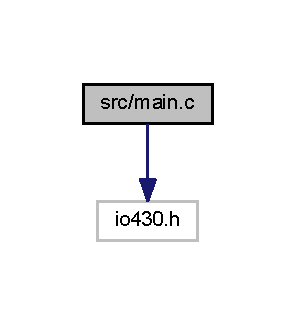
\includegraphics[width=350pt]{main_8c__incl}
\end{center}
\end{figure}
\subsection*{Functions}
\begin{DoxyCompactItemize}
\item 
int \hyperlink{main_8c_a840291bc02cba5474a4cb46a9b9566fe}{main} (void)
\item 
void \hyperlink{main_8c_a471f177dfdefd35621d02eea75c3f6d6}{Error\+Handler} (\hyperlink{types_8h_a0ceed739f3b2b55ee8d4d2a79a82cdea}{u32} Err\+Num)
\begin{DoxyCompactList}\small\item\em Blinkes the error and restarts S\+I\+M900. \end{DoxyCompactList}\item 
void \hyperlink{main_8c_afc3855c9d4720a0bc37839912655a51b}{Ok\+Status\+\_\+\+Update} (void)
\begin{DoxyCompactList}\small\item\em Updates global O\+K-\/flag and turns on the L\+E\+D. \end{DoxyCompactList}\item 
void \hyperlink{main_8c_addd5924d71057cfa18f55f84acf743de}{Sys\+Timer\+\_\+\+Start} (\hyperlink{types_8h_a482359d73191c2bd0ce23a8d9b8f523f}{u16} timeout)
\begin{DoxyCompactList}\small\item\em Starts 150ms system timer, enables interrupt uppon timer every 150ms. \end{DoxyCompactList}\item 
\+\_\+\+\_\+interrupt void \hyperlink{main_8c_ad1a4adc0c6240eb3e90e902dd11ed467}{T\+I\+M\+E\+R1\+\_\+\+A1\+\_\+\+I\+S\+R} (void)
\begin{DoxyCompactList}\small\item\em T\+I\+M\+E\+R\+\_\+\+A1 I\+S\+R counts down timeouts in the system. \end{DoxyCompactList}\item 
void \hyperlink{main_8c_ac5fdf3b2940157c9d81b8a938a279eae}{Send\+Cmd} (\hyperlink{types_8h_aed742c436da53c1080638ce6ef7d13de}{u8} cmd)
\begin{DoxyCompactList}\small\item\em The function sends 1 byte command to a main Water\+Leak controller. \end{DoxyCompactList}\item 
void \hyperlink{main_8c_a7ce0a14b6e7779fbb2d9a05333792c41}{Init} (void)
\begin{DoxyCompactList}\small\item\em M\+C\+U peripheral initialization. \end{DoxyCompactList}\item 
\hyperlink{types_8h_aed742c436da53c1080638ce6ef7d13de}{u8} \hyperlink{main_8c_ae4ce845498558ce8962f23b80045e72d}{C\+R\+C\+\_\+\+Calc} (\hyperlink{types_8h_aed742c436da53c1080638ce6ef7d13de}{u8} $\ast$src, \hyperlink{types_8h_a482359d73191c2bd0ce23a8d9b8f523f}{u16} num)
\begin{DoxyCompactList}\small\item\em Calculates simple control sum via X\+O\+R with 0x\+A\+A. \end{DoxyCompactList}\item 
void \hyperlink{main_8c_ad6c3dd7111bf701431f13cbce565b874}{M\+S\+P430\+\_\+\+U\+C\+S\+\_\+\+Init} (void)
\begin{DoxyCompactList}\small\item\em Configures U\+C\+S for G\+S\+M\+E2 needs. \end{DoxyCompactList}\end{DoxyCompactItemize}
\subsection*{Variables}
\begin{DoxyCompactItemize}
\item 
struct \hyperlink{struct_state___type_def}{State\+\_\+\+Type\+Def} \hyperlink{main_8c_a8fffca79f23706b77ec688ec9144fbf2}{State}
\item 
struct \hyperlink{struct_in_pack___type_def}{In\+Pack\+\_\+\+Type\+Def} \hyperlink{main_8c_a1e355aed5ee123977647172c50a0b50b}{In\+Pack}
\item 
struct \hyperlink{struct_out_pack___type_def}{Out\+Pack\+\_\+\+Type\+Def} \hyperlink{main_8c_a13cd5ce063acb4886ef8b13cdf215d0a}{Out\+Pack}
\end{DoxyCompactItemize}


\subsection{Function Documentation}
\hypertarget{main_8c_ae4ce845498558ce8962f23b80045e72d}{}\index{main.\+c@{main.\+c}!C\+R\+C\+\_\+\+Calc@{C\+R\+C\+\_\+\+Calc}}
\index{C\+R\+C\+\_\+\+Calc@{C\+R\+C\+\_\+\+Calc}!main.\+c@{main.\+c}}
\subsubsection[{C\+R\+C\+\_\+\+Calc}]{\setlength{\rightskip}{0pt plus 5cm}{\bf u8} C\+R\+C\+\_\+\+Calc (
\begin{DoxyParamCaption}
\item[{{\bf u8} $\ast$}]{src, }
\item[{{\bf u16}}]{num}
\end{DoxyParamCaption}
)}\label{main_8c_ae4ce845498558ce8962f23b80045e72d}


Calculates simple control sum via X\+O\+R with 0x\+A\+A. 



Definition at line 260 of file main.\+c.



Here is the caller graph for this function\+:
\nopagebreak
\begin{figure}[H]
\begin{center}
\leavevmode
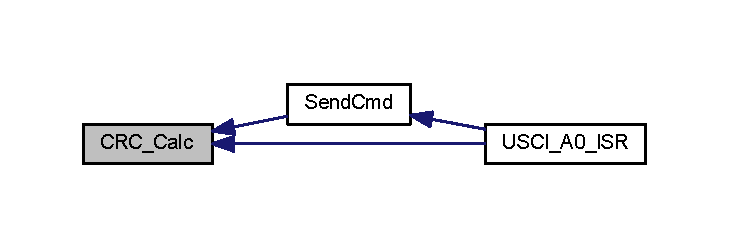
\includegraphics[width=350pt]{main_8c_ae4ce845498558ce8962f23b80045e72d_icgraph}
\end{center}
\end{figure}


\hypertarget{main_8c_a471f177dfdefd35621d02eea75c3f6d6}{}\index{main.\+c@{main.\+c}!Error\+Handler@{Error\+Handler}}
\index{Error\+Handler@{Error\+Handler}!main.\+c@{main.\+c}}
\subsubsection[{Error\+Handler}]{\setlength{\rightskip}{0pt plus 5cm}void Error\+Handler (
\begin{DoxyParamCaption}
\item[{{\bf u32}}]{Err\+Num}
\end{DoxyParamCaption}
)}\label{main_8c_a471f177dfdefd35621d02eea75c3f6d6}


Blinkes the error and restarts S\+I\+M900. 

The function blinks out the number of the error by the L\+E\+D. 

Definition at line 91 of file main.\+c.



Here is the call graph for this function\+:
\nopagebreak
\begin{figure}[H]
\begin{center}
\leavevmode
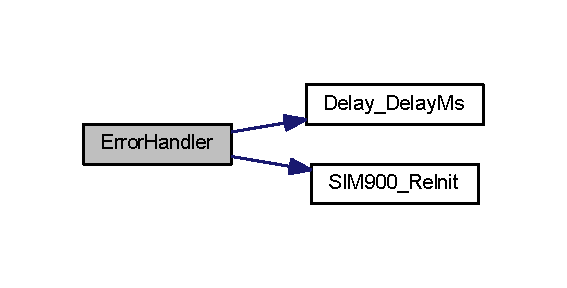
\includegraphics[width=272pt]{main_8c_a471f177dfdefd35621d02eea75c3f6d6_cgraph}
\end{center}
\end{figure}




Here is the caller graph for this function\+:
\nopagebreak
\begin{figure}[H]
\begin{center}
\leavevmode
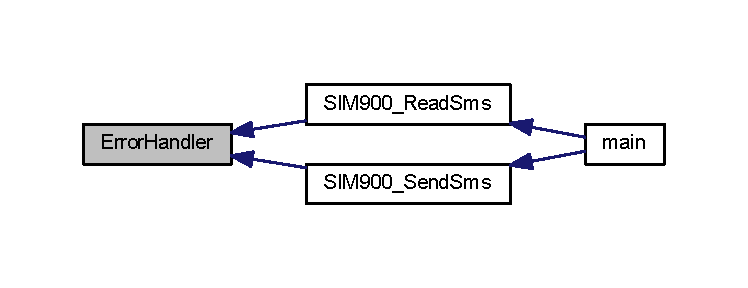
\includegraphics[width=350pt]{main_8c_a471f177dfdefd35621d02eea75c3f6d6_icgraph}
\end{center}
\end{figure}


\hypertarget{main_8c_a7ce0a14b6e7779fbb2d9a05333792c41}{}\index{main.\+c@{main.\+c}!Init@{Init}}
\index{Init@{Init}!main.\+c@{main.\+c}}
\subsubsection[{Init}]{\setlength{\rightskip}{0pt plus 5cm}void Init (
\begin{DoxyParamCaption}
\item[{void}]{}
\end{DoxyParamCaption}
)}\label{main_8c_a7ce0a14b6e7779fbb2d9a05333792c41}


M\+C\+U peripheral initialization. 

The function configures the following modules\+:
\begin{DoxyEnumerate}
\item U\+S\+C\+I\+\_\+\+A\+O for R\+S-\/485 communication
\item U\+S\+C\+I\+\_\+\+A1 for S\+I\+M900 communication
\item G\+P\+I\+O 3.\+1 Power switch pin for S\+I\+M900 3.\+2 Off/on S\+I\+M900 pin 3.\+3 Input pin to obtain S\+I\+M900 status 3.\+4 R\textbackslash{} R\+S485 (Toggling between Rx and Tx) 3.\+5 L\+E\+D pin initialization
\item Delay module initialization
\item S\+M\+S Queue module initialization
\item Talephone Directory module initialzation
\item Power measurements initialization
\item S\+I\+M900 Start
\item Main timer start 
\end{DoxyEnumerate}

Definition at line 239 of file main.\+c.



Here is the call graph for this function\+:
\nopagebreak
\begin{figure}[H]
\begin{center}
\leavevmode
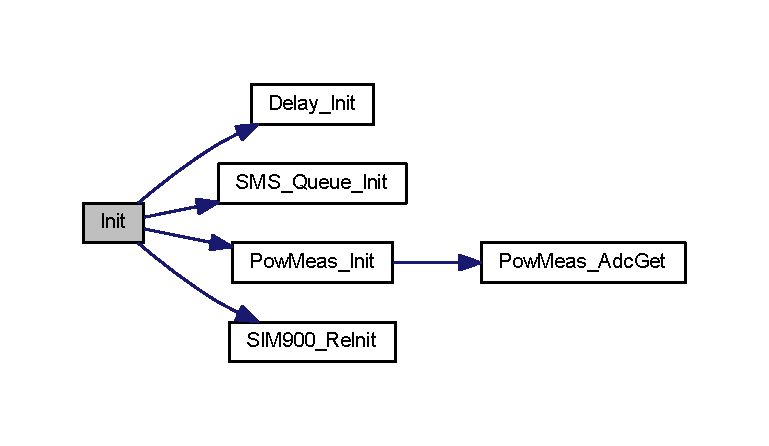
\includegraphics[width=350pt]{main_8c_a7ce0a14b6e7779fbb2d9a05333792c41_cgraph}
\end{center}
\end{figure}




Here is the caller graph for this function\+:
\nopagebreak
\begin{figure}[H]
\begin{center}
\leavevmode
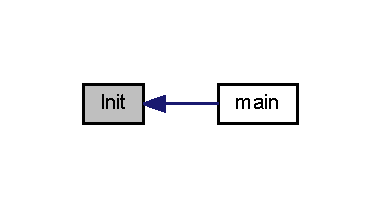
\includegraphics[width=183pt]{main_8c_a7ce0a14b6e7779fbb2d9a05333792c41_icgraph}
\end{center}
\end{figure}


\hypertarget{main_8c_a840291bc02cba5474a4cb46a9b9566fe}{}\index{main.\+c@{main.\+c}!main@{main}}
\index{main@{main}!main.\+c@{main.\+c}}
\subsubsection[{main}]{\setlength{\rightskip}{0pt plus 5cm}int main (
\begin{DoxyParamCaption}
\item[{void}]{}
\end{DoxyParamCaption}
)}\label{main_8c_a840291bc02cba5474a4cb46a9b9566fe}


Definition at line 7 of file main.\+c.



Here is the call graph for this function\+:
\nopagebreak
\begin{figure}[H]
\begin{center}
\leavevmode
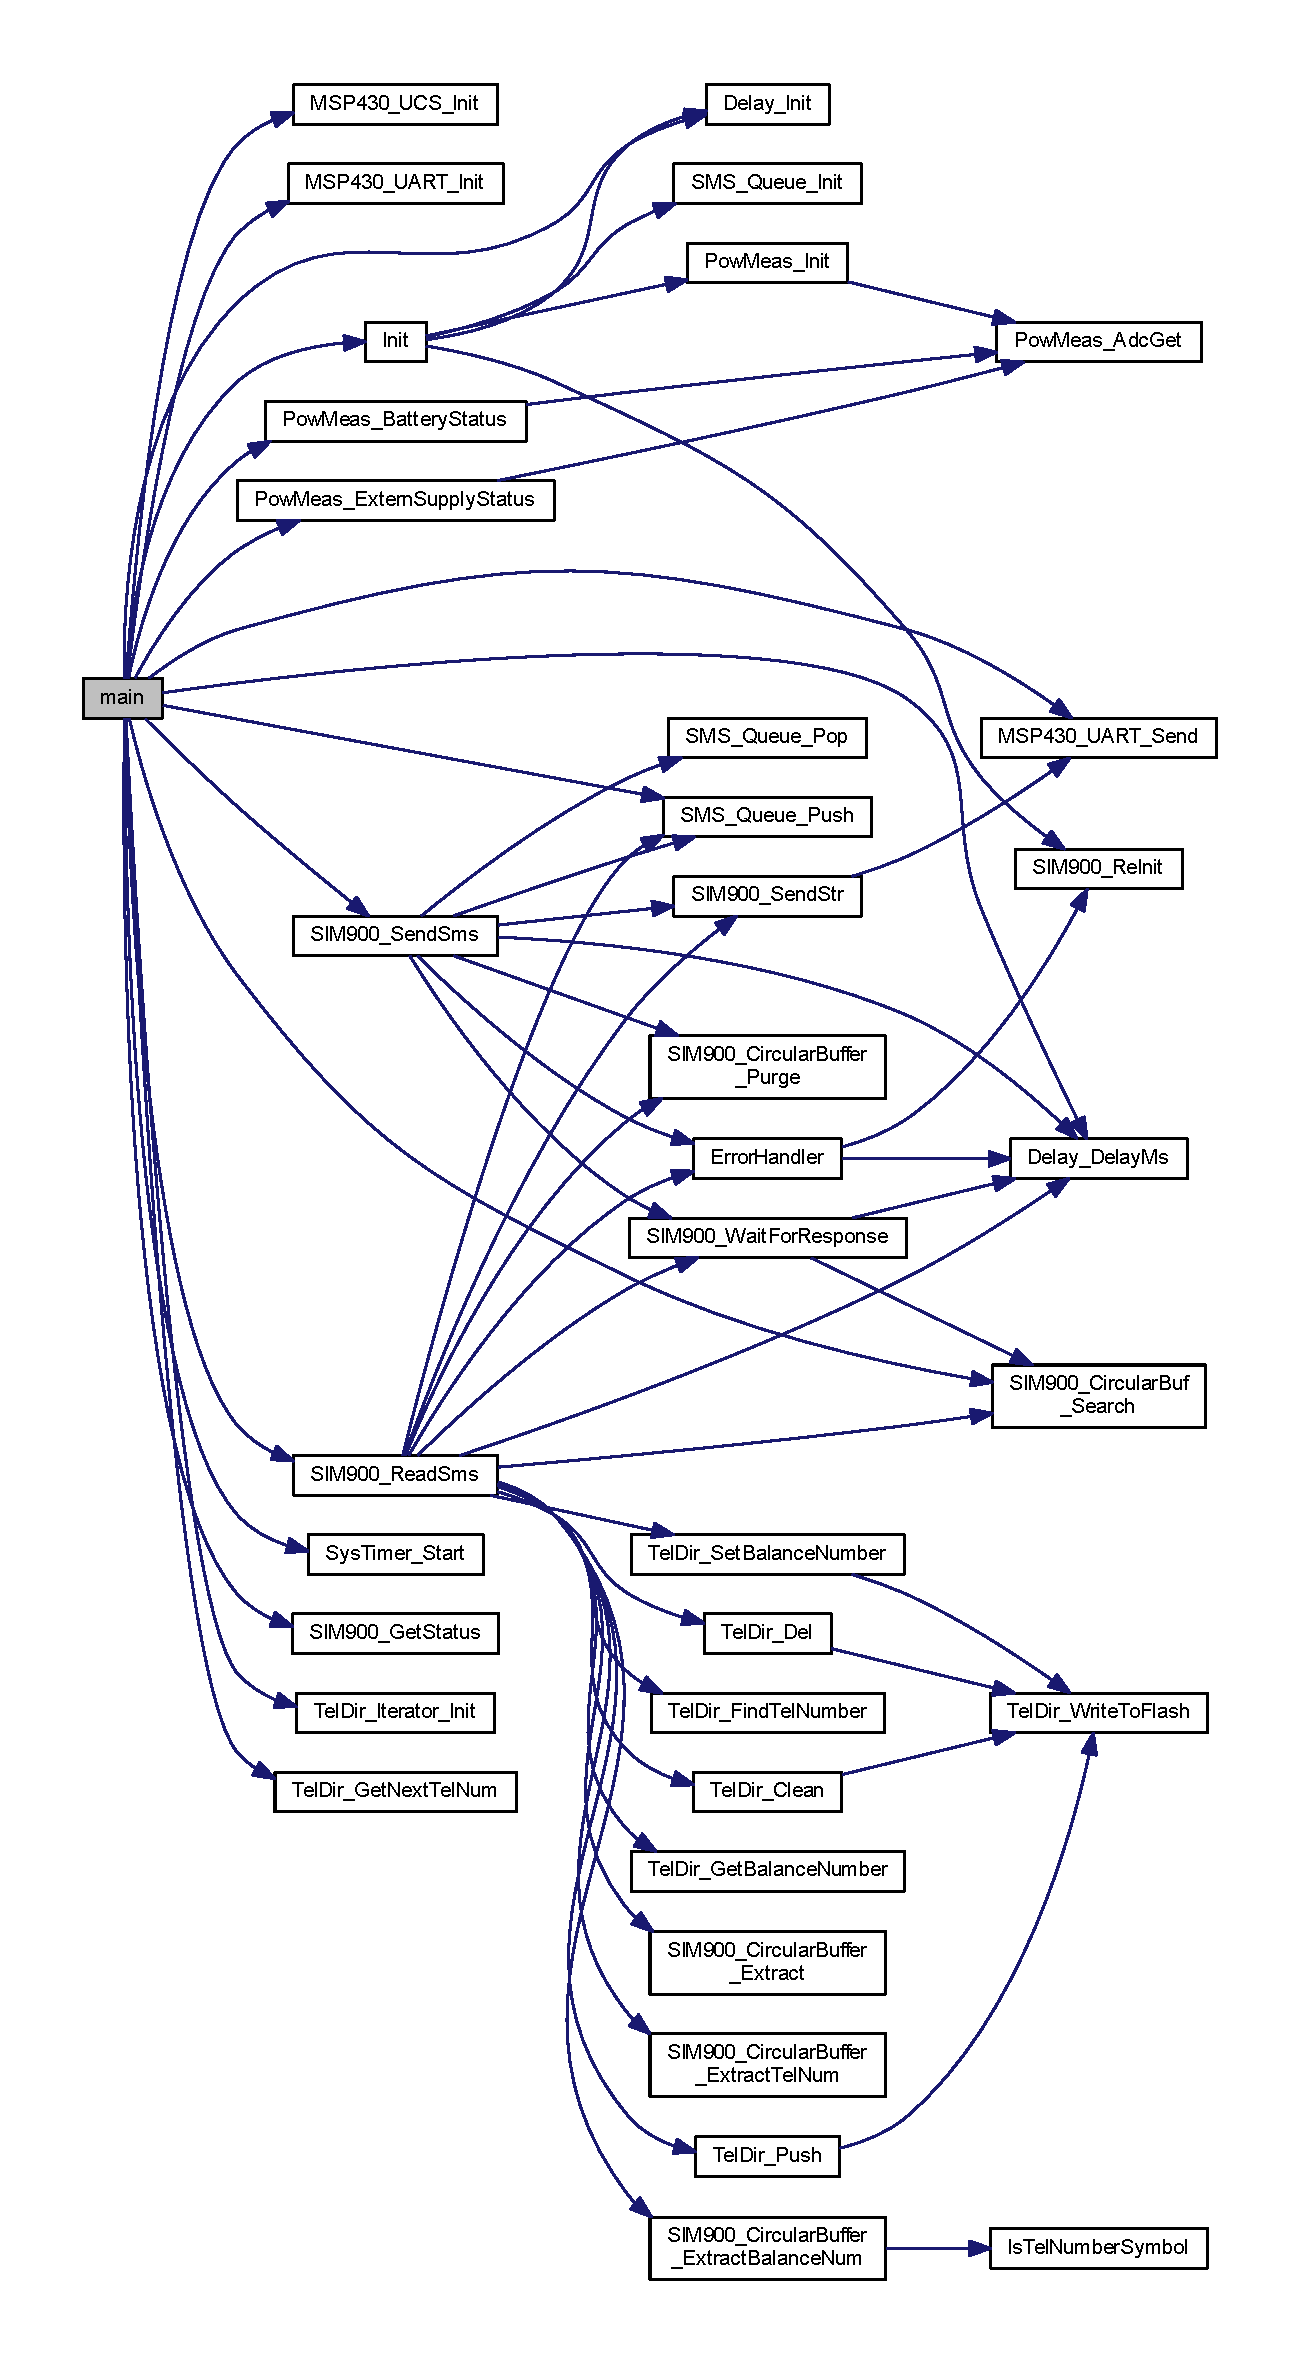
\includegraphics[height=550pt]{main_8c_a840291bc02cba5474a4cb46a9b9566fe_cgraph}
\end{center}
\end{figure}


\hypertarget{main_8c_ad6c3dd7111bf701431f13cbce565b874}{}\index{main.\+c@{main.\+c}!M\+S\+P430\+\_\+\+U\+C\+S\+\_\+\+Init@{M\+S\+P430\+\_\+\+U\+C\+S\+\_\+\+Init}}
\index{M\+S\+P430\+\_\+\+U\+C\+S\+\_\+\+Init@{M\+S\+P430\+\_\+\+U\+C\+S\+\_\+\+Init}!main.\+c@{main.\+c}}
\subsubsection[{M\+S\+P430\+\_\+\+U\+C\+S\+\_\+\+Init}]{\setlength{\rightskip}{0pt plus 5cm}void M\+S\+P430\+\_\+\+U\+C\+S\+\_\+\+Init (
\begin{DoxyParamCaption}
\item[{void}]{}
\end{DoxyParamCaption}
)}\label{main_8c_ad6c3dd7111bf701431f13cbce565b874}


Configures U\+C\+S for G\+S\+M\+E2 needs. 

The function sets D\+C\+O\+C\+L\+K and D\+C\+O\+C\+L\+K\+D\+I\+V to 25\+M\+Hz

Source clock for F\+F\+L\+: R\+E\+F\+O\+C\+L\+K 32768\+Hz F\+L\+L\+R\+E\+F\+D\+I\+V = 1 F\+L\+L\+N = 762 D\+C\+O\+R\+S\+E\+L = 6 D\+C\+O = 15 F\+L\+L\+D = 1 

Definition at line 278 of file main.\+c.



Here is the caller graph for this function\+:
\nopagebreak
\begin{figure}[H]
\begin{center}
\leavevmode
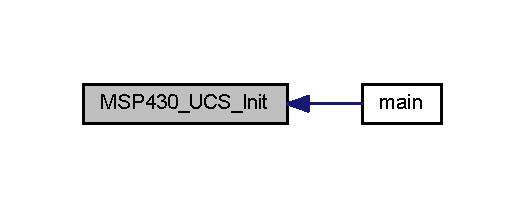
\includegraphics[width=252pt]{main_8c_ad6c3dd7111bf701431f13cbce565b874_icgraph}
\end{center}
\end{figure}


\hypertarget{main_8c_afc3855c9d4720a0bc37839912655a51b}{}\index{main.\+c@{main.\+c}!Ok\+Status\+\_\+\+Update@{Ok\+Status\+\_\+\+Update}}
\index{Ok\+Status\+\_\+\+Update@{Ok\+Status\+\_\+\+Update}!main.\+c@{main.\+c}}
\subsubsection[{Ok\+Status\+\_\+\+Update}]{\setlength{\rightskip}{0pt plus 5cm}void Ok\+Status\+\_\+\+Update (
\begin{DoxyParamCaption}
\item[{void}]{}
\end{DoxyParamCaption}
)}\label{main_8c_afc3855c9d4720a0bc37839912655a51b}


Updates global O\+K-\/flag and turns on the L\+E\+D. 



Definition at line 111 of file main.\+c.



Here is the caller graph for this function\+:
\nopagebreak
\begin{figure}[H]
\begin{center}
\leavevmode
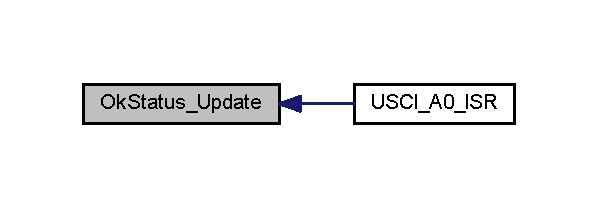
\includegraphics[width=287pt]{main_8c_afc3855c9d4720a0bc37839912655a51b_icgraph}
\end{center}
\end{figure}


\hypertarget{main_8c_ac5fdf3b2940157c9d81b8a938a279eae}{}\index{main.\+c@{main.\+c}!Send\+Cmd@{Send\+Cmd}}
\index{Send\+Cmd@{Send\+Cmd}!main.\+c@{main.\+c}}
\subsubsection[{Send\+Cmd}]{\setlength{\rightskip}{0pt plus 5cm}void Send\+Cmd (
\begin{DoxyParamCaption}
\item[{{\bf u8}}]{cmd}
\end{DoxyParamCaption}
)}\label{main_8c_ac5fdf3b2940157c9d81b8a938a279eae}


The function sends 1 byte command to a main Water\+Leak controller. 

The function builds the outgoing packet, calculates the check sum and sends all that. 

Definition at line 192 of file main.\+c.



Here is the call graph for this function\+:
\nopagebreak
\begin{figure}[H]
\begin{center}
\leavevmode
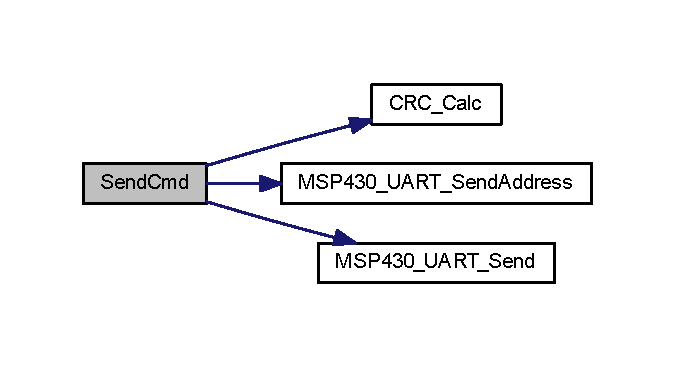
\includegraphics[width=324pt]{main_8c_ac5fdf3b2940157c9d81b8a938a279eae_cgraph}
\end{center}
\end{figure}




Here is the caller graph for this function\+:
\nopagebreak
\begin{figure}[H]
\begin{center}
\leavevmode
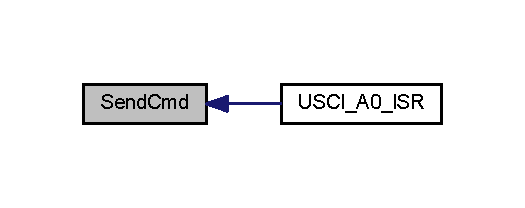
\includegraphics[width=252pt]{main_8c_ac5fdf3b2940157c9d81b8a938a279eae_icgraph}
\end{center}
\end{figure}


\hypertarget{main_8c_addd5924d71057cfa18f55f84acf743de}{}\index{main.\+c@{main.\+c}!Sys\+Timer\+\_\+\+Start@{Sys\+Timer\+\_\+\+Start}}
\index{Sys\+Timer\+\_\+\+Start@{Sys\+Timer\+\_\+\+Start}!main.\+c@{main.\+c}}
\subsubsection[{Sys\+Timer\+\_\+\+Start}]{\setlength{\rightskip}{0pt plus 5cm}void Sys\+Timer\+\_\+\+Start (
\begin{DoxyParamCaption}
\item[{{\bf u16}}]{timeout}
\end{DoxyParamCaption}
)}\label{main_8c_addd5924d71057cfa18f55f84acf743de}


Starts 150ms system timer, enables interrupt uppon timer every 150ms. 



Definition at line 119 of file main.\+c.



Here is the caller graph for this function\+:
\nopagebreak
\begin{figure}[H]
\begin{center}
\leavevmode
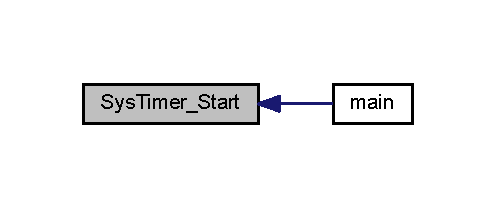
\includegraphics[width=238pt]{main_8c_addd5924d71057cfa18f55f84acf743de_icgraph}
\end{center}
\end{figure}


\hypertarget{main_8c_ad1a4adc0c6240eb3e90e902dd11ed467}{}\index{main.\+c@{main.\+c}!T\+I\+M\+E\+R1\+\_\+\+A1\+\_\+\+I\+S\+R@{T\+I\+M\+E\+R1\+\_\+\+A1\+\_\+\+I\+S\+R}}
\index{T\+I\+M\+E\+R1\+\_\+\+A1\+\_\+\+I\+S\+R@{T\+I\+M\+E\+R1\+\_\+\+A1\+\_\+\+I\+S\+R}!main.\+c@{main.\+c}}
\subsubsection[{T\+I\+M\+E\+R1\+\_\+\+A1\+\_\+\+I\+S\+R}]{\setlength{\rightskip}{0pt plus 5cm}\+\_\+\+\_\+interrupt void T\+I\+M\+E\+R1\+\_\+\+A1\+\_\+\+I\+S\+R (
\begin{DoxyParamCaption}
\item[{void}]{}
\end{DoxyParamCaption}
)}\label{main_8c_ad1a4adc0c6240eb3e90e902dd11ed467}


T\+I\+M\+E\+R\+\_\+\+A1 I\+S\+R counts down timeouts in the system. 

The timer catches several timeouts.


\begin{DoxyEnumerate}
\item Close Valves Timeout This timeout is set when command to close all valves received and the timeout is being expired until acknoledgement of succesful command execution gotten.
\item Open Valves Timeout This timeout is set when command to open all valves received and the timeout is being expired until acknoledgement of succesful command execution gotten.
\item O\+K Timeout This timeout is reset each time Water\+Leak controller riches us. If timeout eventually expired that\textquotesingle{}s concerned as the Water\+Leak controller lost. 
\end{DoxyEnumerate}

Definition at line 150 of file main.\+c.



Here is the call graph for this function\+:
\nopagebreak
\begin{figure}[H]
\begin{center}
\leavevmode
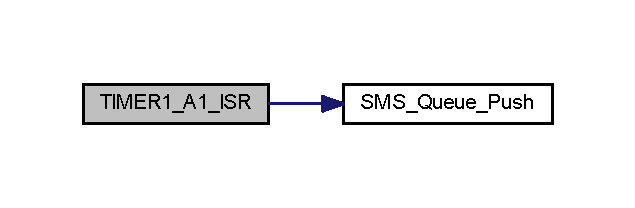
\includegraphics[width=305pt]{main_8c_ad1a4adc0c6240eb3e90e902dd11ed467_cgraph}
\end{center}
\end{figure}




\subsection{Variable Documentation}
\hypertarget{main_8c_a1e355aed5ee123977647172c50a0b50b}{}\index{main.\+c@{main.\+c}!In\+Pack@{In\+Pack}}
\index{In\+Pack@{In\+Pack}!main.\+c@{main.\+c}}
\subsubsection[{In\+Pack}]{\setlength{\rightskip}{0pt plus 5cm}struct {\bf In\+Pack\+\_\+\+Type\+Def} In\+Pack}\label{main_8c_a1e355aed5ee123977647172c50a0b50b}


Definition at line 4 of file main.\+c.

\hypertarget{main_8c_a13cd5ce063acb4886ef8b13cdf215d0a}{}\index{main.\+c@{main.\+c}!Out\+Pack@{Out\+Pack}}
\index{Out\+Pack@{Out\+Pack}!main.\+c@{main.\+c}}
\subsubsection[{Out\+Pack}]{\setlength{\rightskip}{0pt plus 5cm}struct {\bf Out\+Pack\+\_\+\+Type\+Def} Out\+Pack}\label{main_8c_a13cd5ce063acb4886ef8b13cdf215d0a}


Definition at line 5 of file main.\+c.

\hypertarget{main_8c_a8fffca79f23706b77ec688ec9144fbf2}{}\index{main.\+c@{main.\+c}!State@{State}}
\index{State@{State}!main.\+c@{main.\+c}}
\subsubsection[{State}]{\setlength{\rightskip}{0pt plus 5cm}struct {\bf State\+\_\+\+Type\+Def} State}\label{main_8c_a8fffca79f23706b77ec688ec9144fbf2}


Definition at line 3 of file main.\+c.


%--- End generated contents ---

% Index
\backmatter
\newpage
\phantomsection
\clearemptydoublepage
\addcontentsline{toc}{chapter}{Index}
\printindex

\end{document}
